\documentclass[a4paper,11pt]{article}
\usepackage{graphicx}
\usepackage{booktabs}
\usepackage{setspace}
\usepackage{parskip}
\usepackage[english]{babel}
\usepackage{refstyle}
\usepackage{hyperref}
\usepackage{caption}
\usepackage{subcaption}
\usepackage{amsmath}
\onehalfspacing
\begin{document}

\author{Mario Tambos}
\title{\vspace{-2cm}Report for Sheet 03\\
\small{Lab Course Machine Learning and Data Analysis}}
\maketitle

\section*{Implementation comments}
The code was structured mostly in functions following an imperative paradigm,
except for the \verb|krr| and \verb|SupervisedMethod| classes, which were required by the assignment's statement.

One function was declared for each assignment in Part 2.

Beyond \verb|matplotlib|, \verb|numpy| and \verb|scipy|, \verb|seaborn| was used to improve the plots aesthetics in Part 2.

All tasks were completed, except for the final point of Assignment 4, and all tests passed.
 
\section*{Assignment 3}

\Figref{assignment3} shows the ROC curves for different sample sizes.
The false positive (${fpr}_n$) and true positive (${tpr}_n$) rates for a sample of size $n$ were calculated analytically as follows:

\begin{align*}
	{fpr}_n &= (1 - \Phi(x_0; \mu=0, \sigma^2=1))\\
	{tpr}_n &= (1 - \Phi(x_0; \mu=2, \sigma^2=1))
\end{align*}

where $x_0 \in [-5, 5]$ is the threshold (bias) term.

As seen in the plot, the empirical ROC curve converges to the analytical ROC curve asymptotically.

\begin{figure}
  \centering
  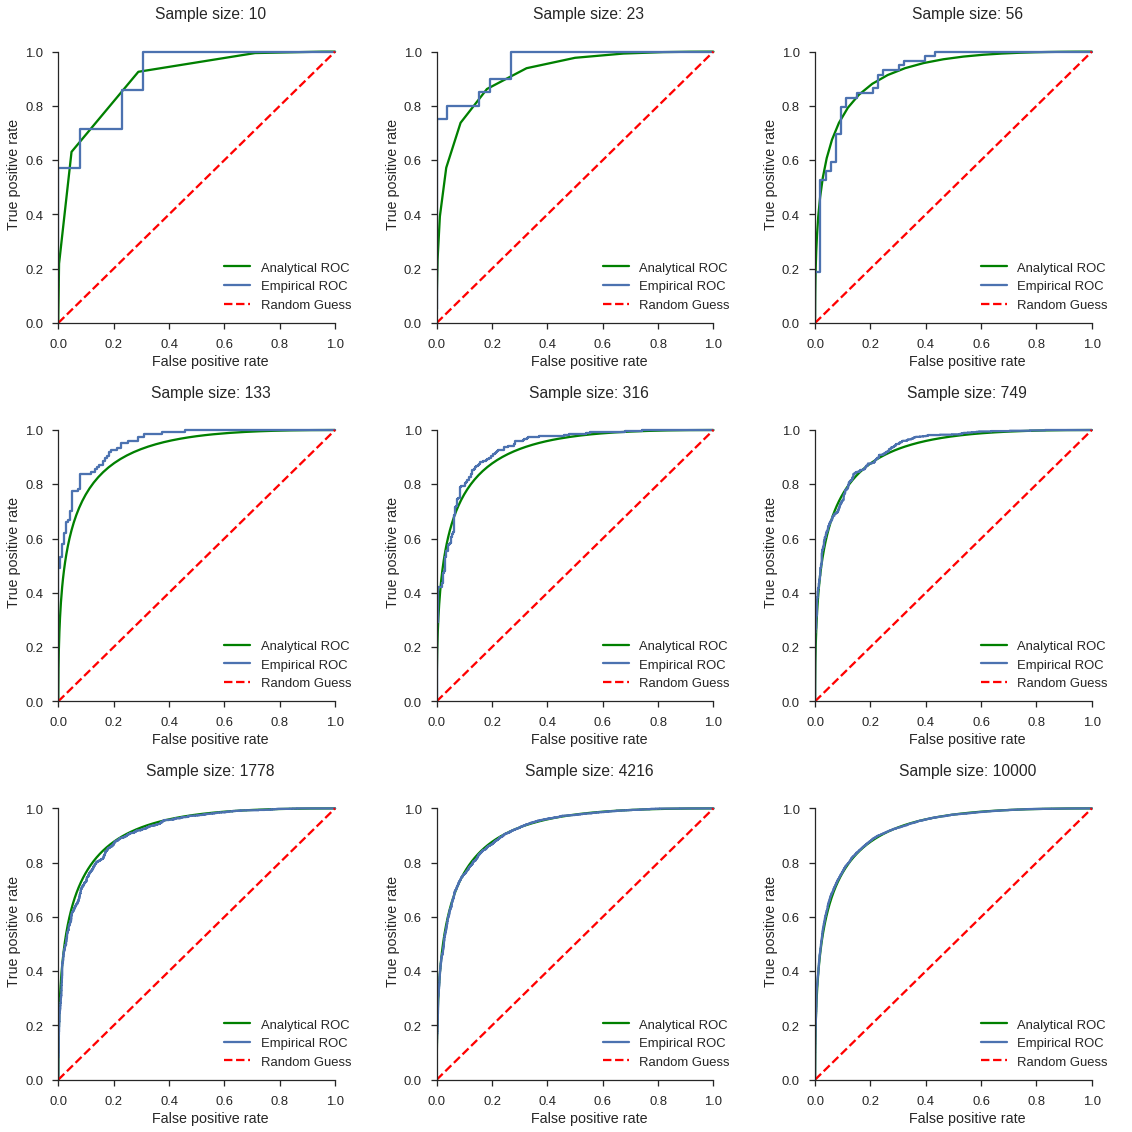
\includegraphics[width=\textwidth]{images/assignment_3.png}
  \caption{Analytical vs empirical ROC curves for different sample sizes.}
  \label{fig:assignment3}
\end{figure}


\section*{Assignment 4}

\Figref{assignment4} shows the ROC curves for the five datasets, with their corresponding AUC scores and cross validation losses.

From the experiments, it would seem that the AUC score has an inverse relationship to the cross validation loss; i.e., larger AUC scores correspond to lower cross validation losses.

\begin{figure}
	\centering
	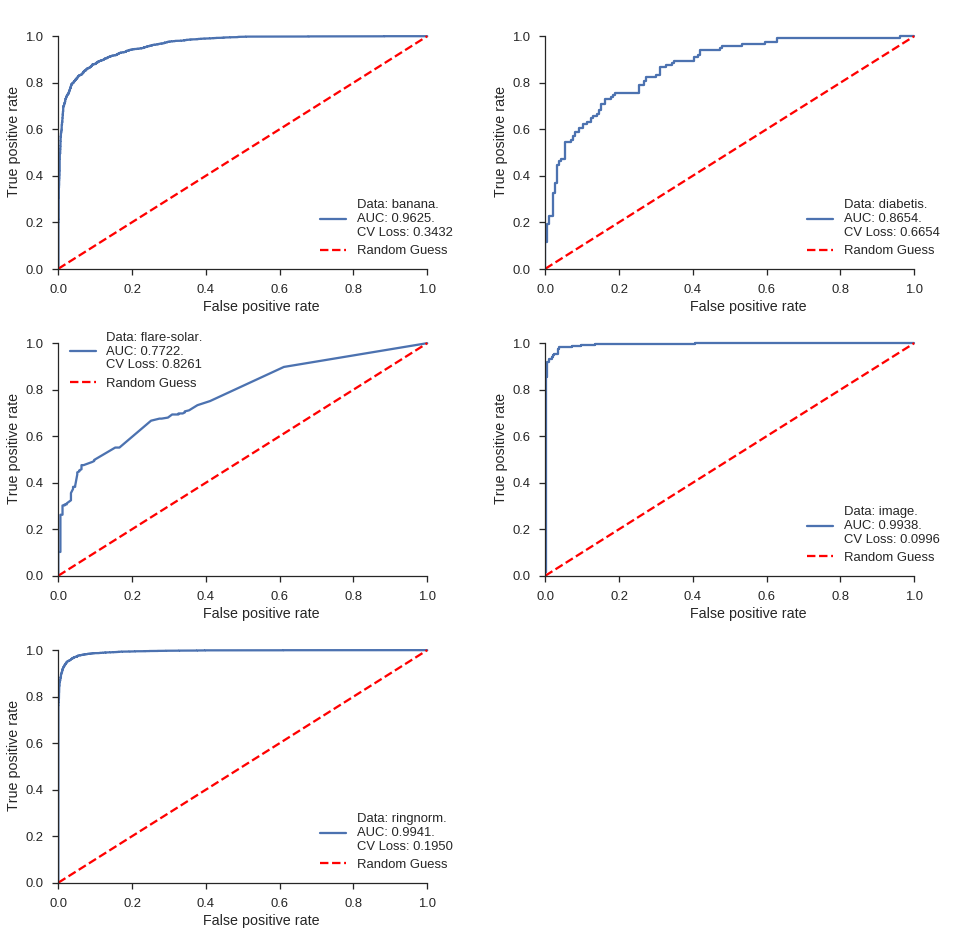
\includegraphics[width=\textwidth]{images/assignment_4.png}
	\caption{ROC curves for KRR resulting from variation of the bias term, with their respective AUC and cross-validation loss values.}
	\label{fig:assignment4}
\end{figure}

\end{document}

